Here you can see how to include an image in your document.
%\begin{sidewaysfigure}
%\centering
%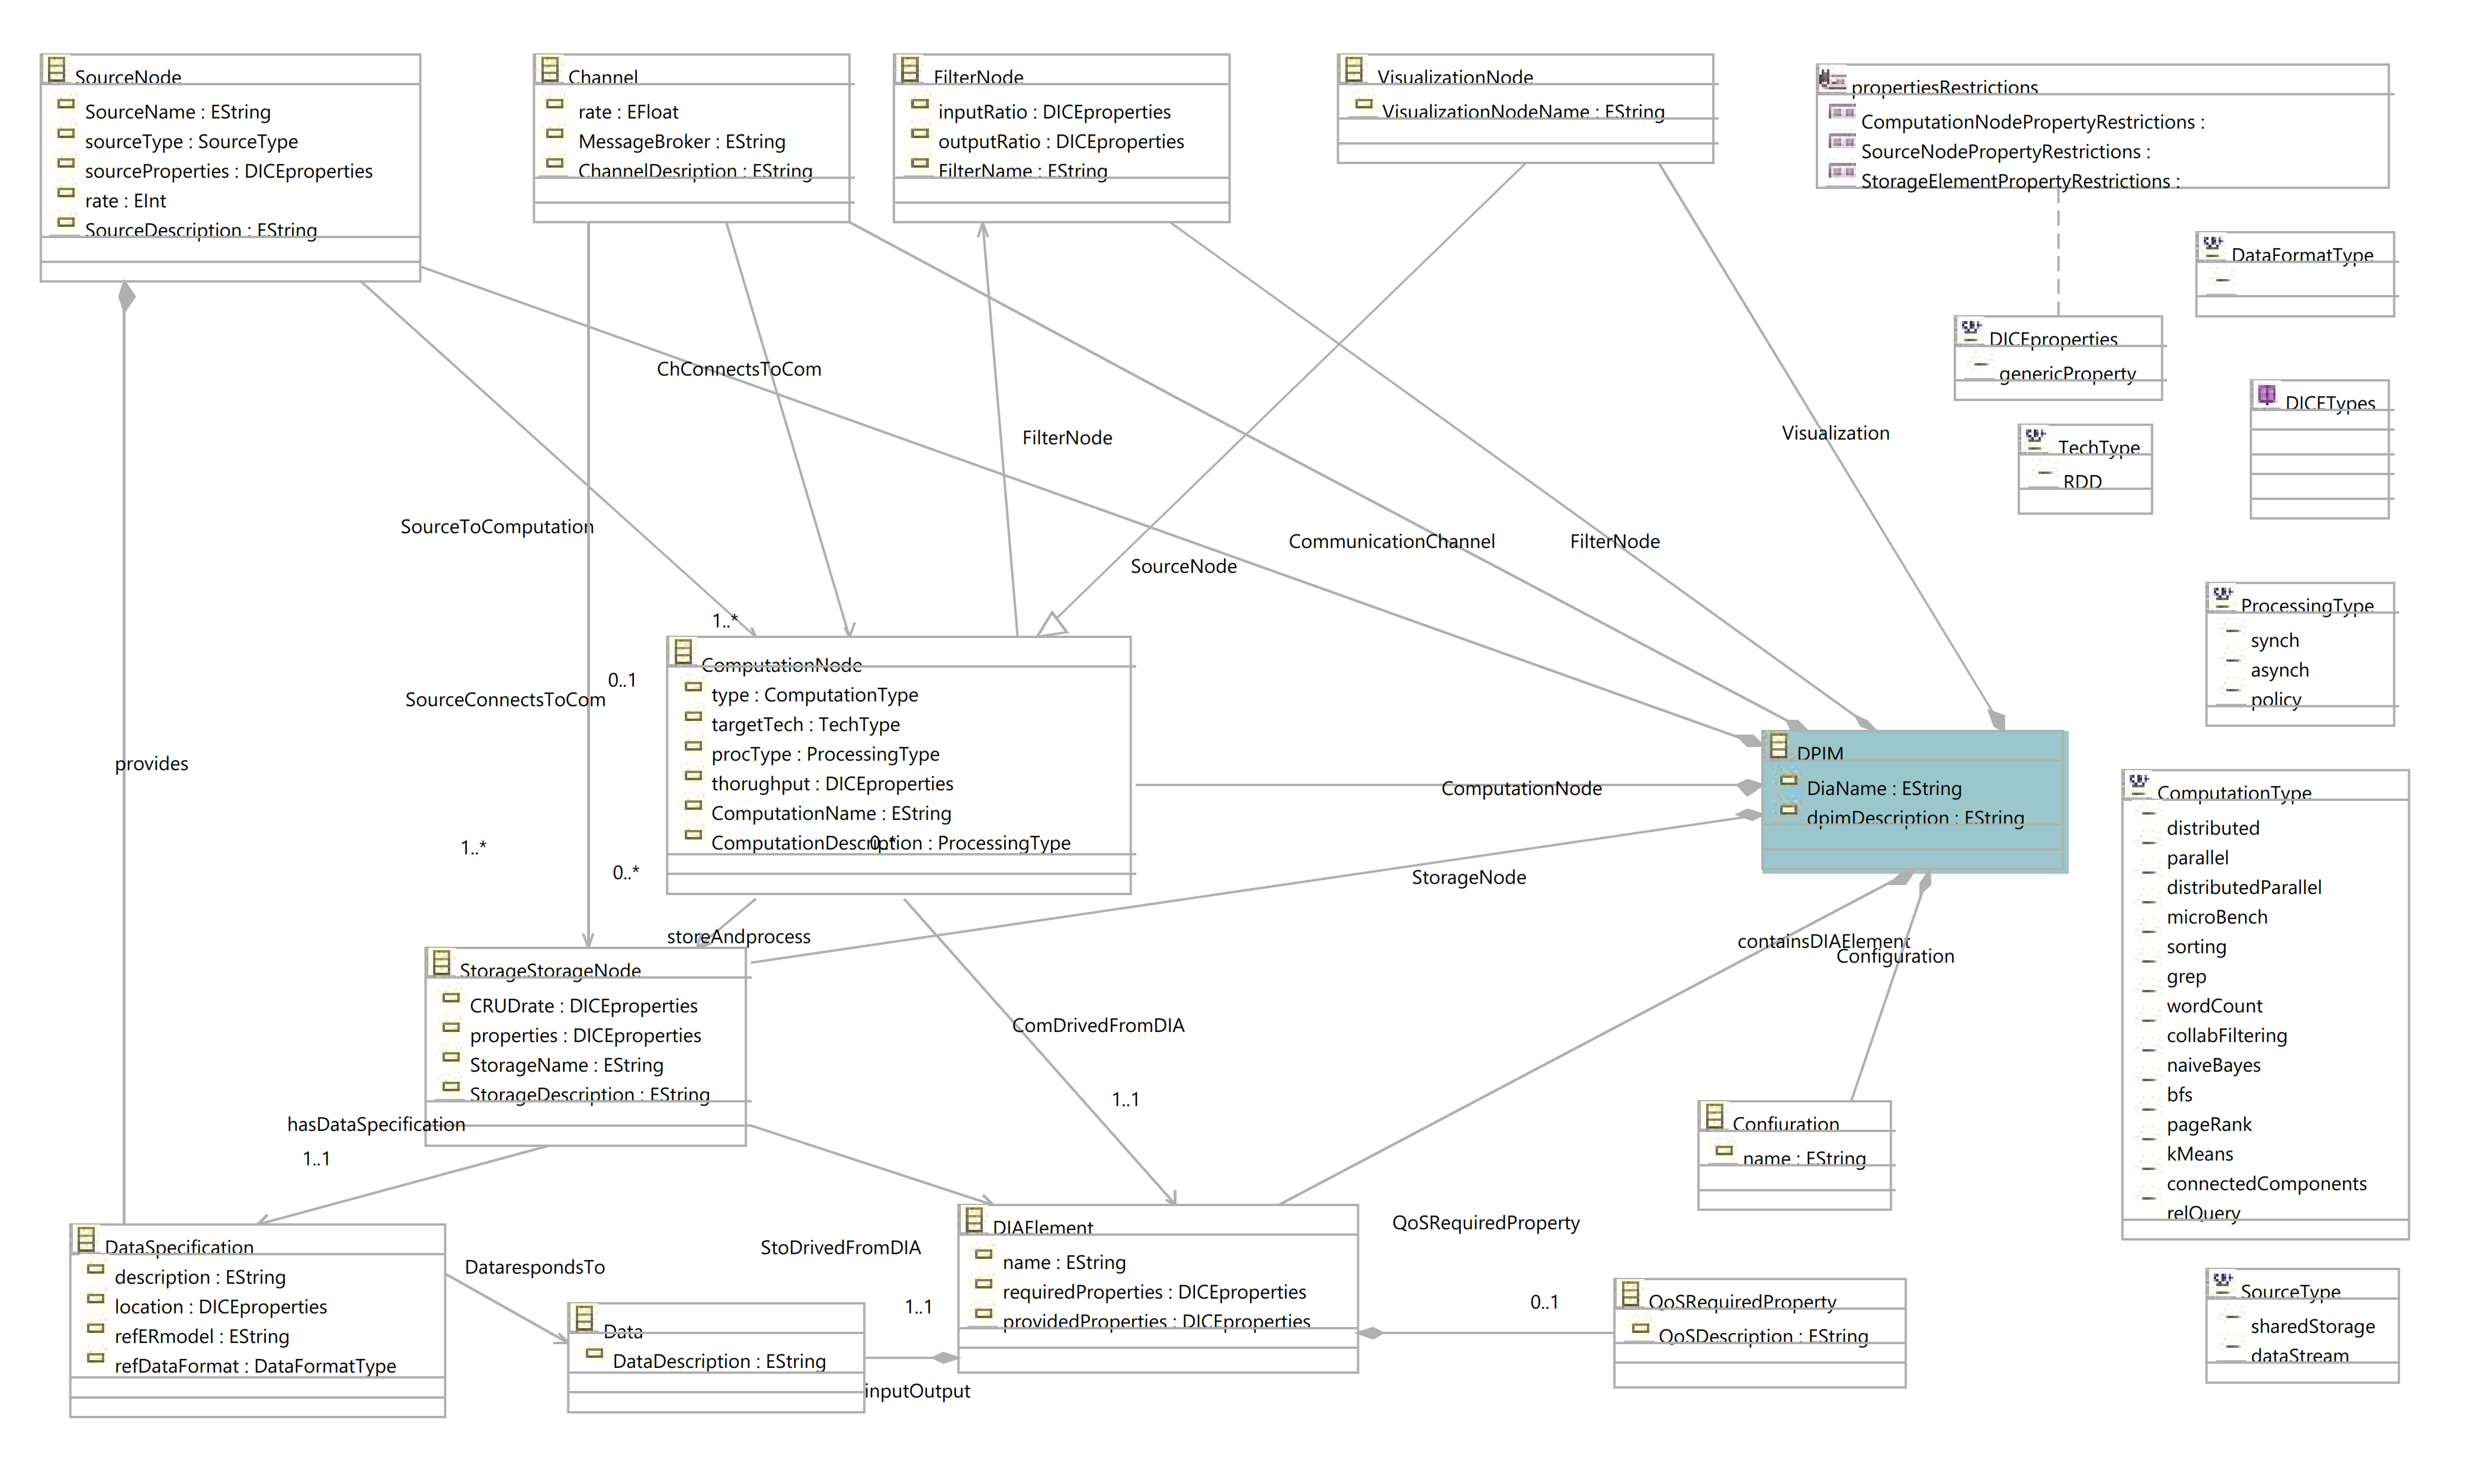
\includegraphics[width=\textwidth]{Images/11.png}
%\caption{\label{fig:metamodel}DICE DPIM metamodel.}
%\end{sidewaysfigure}
%
%\begin{figure}
%\centering
%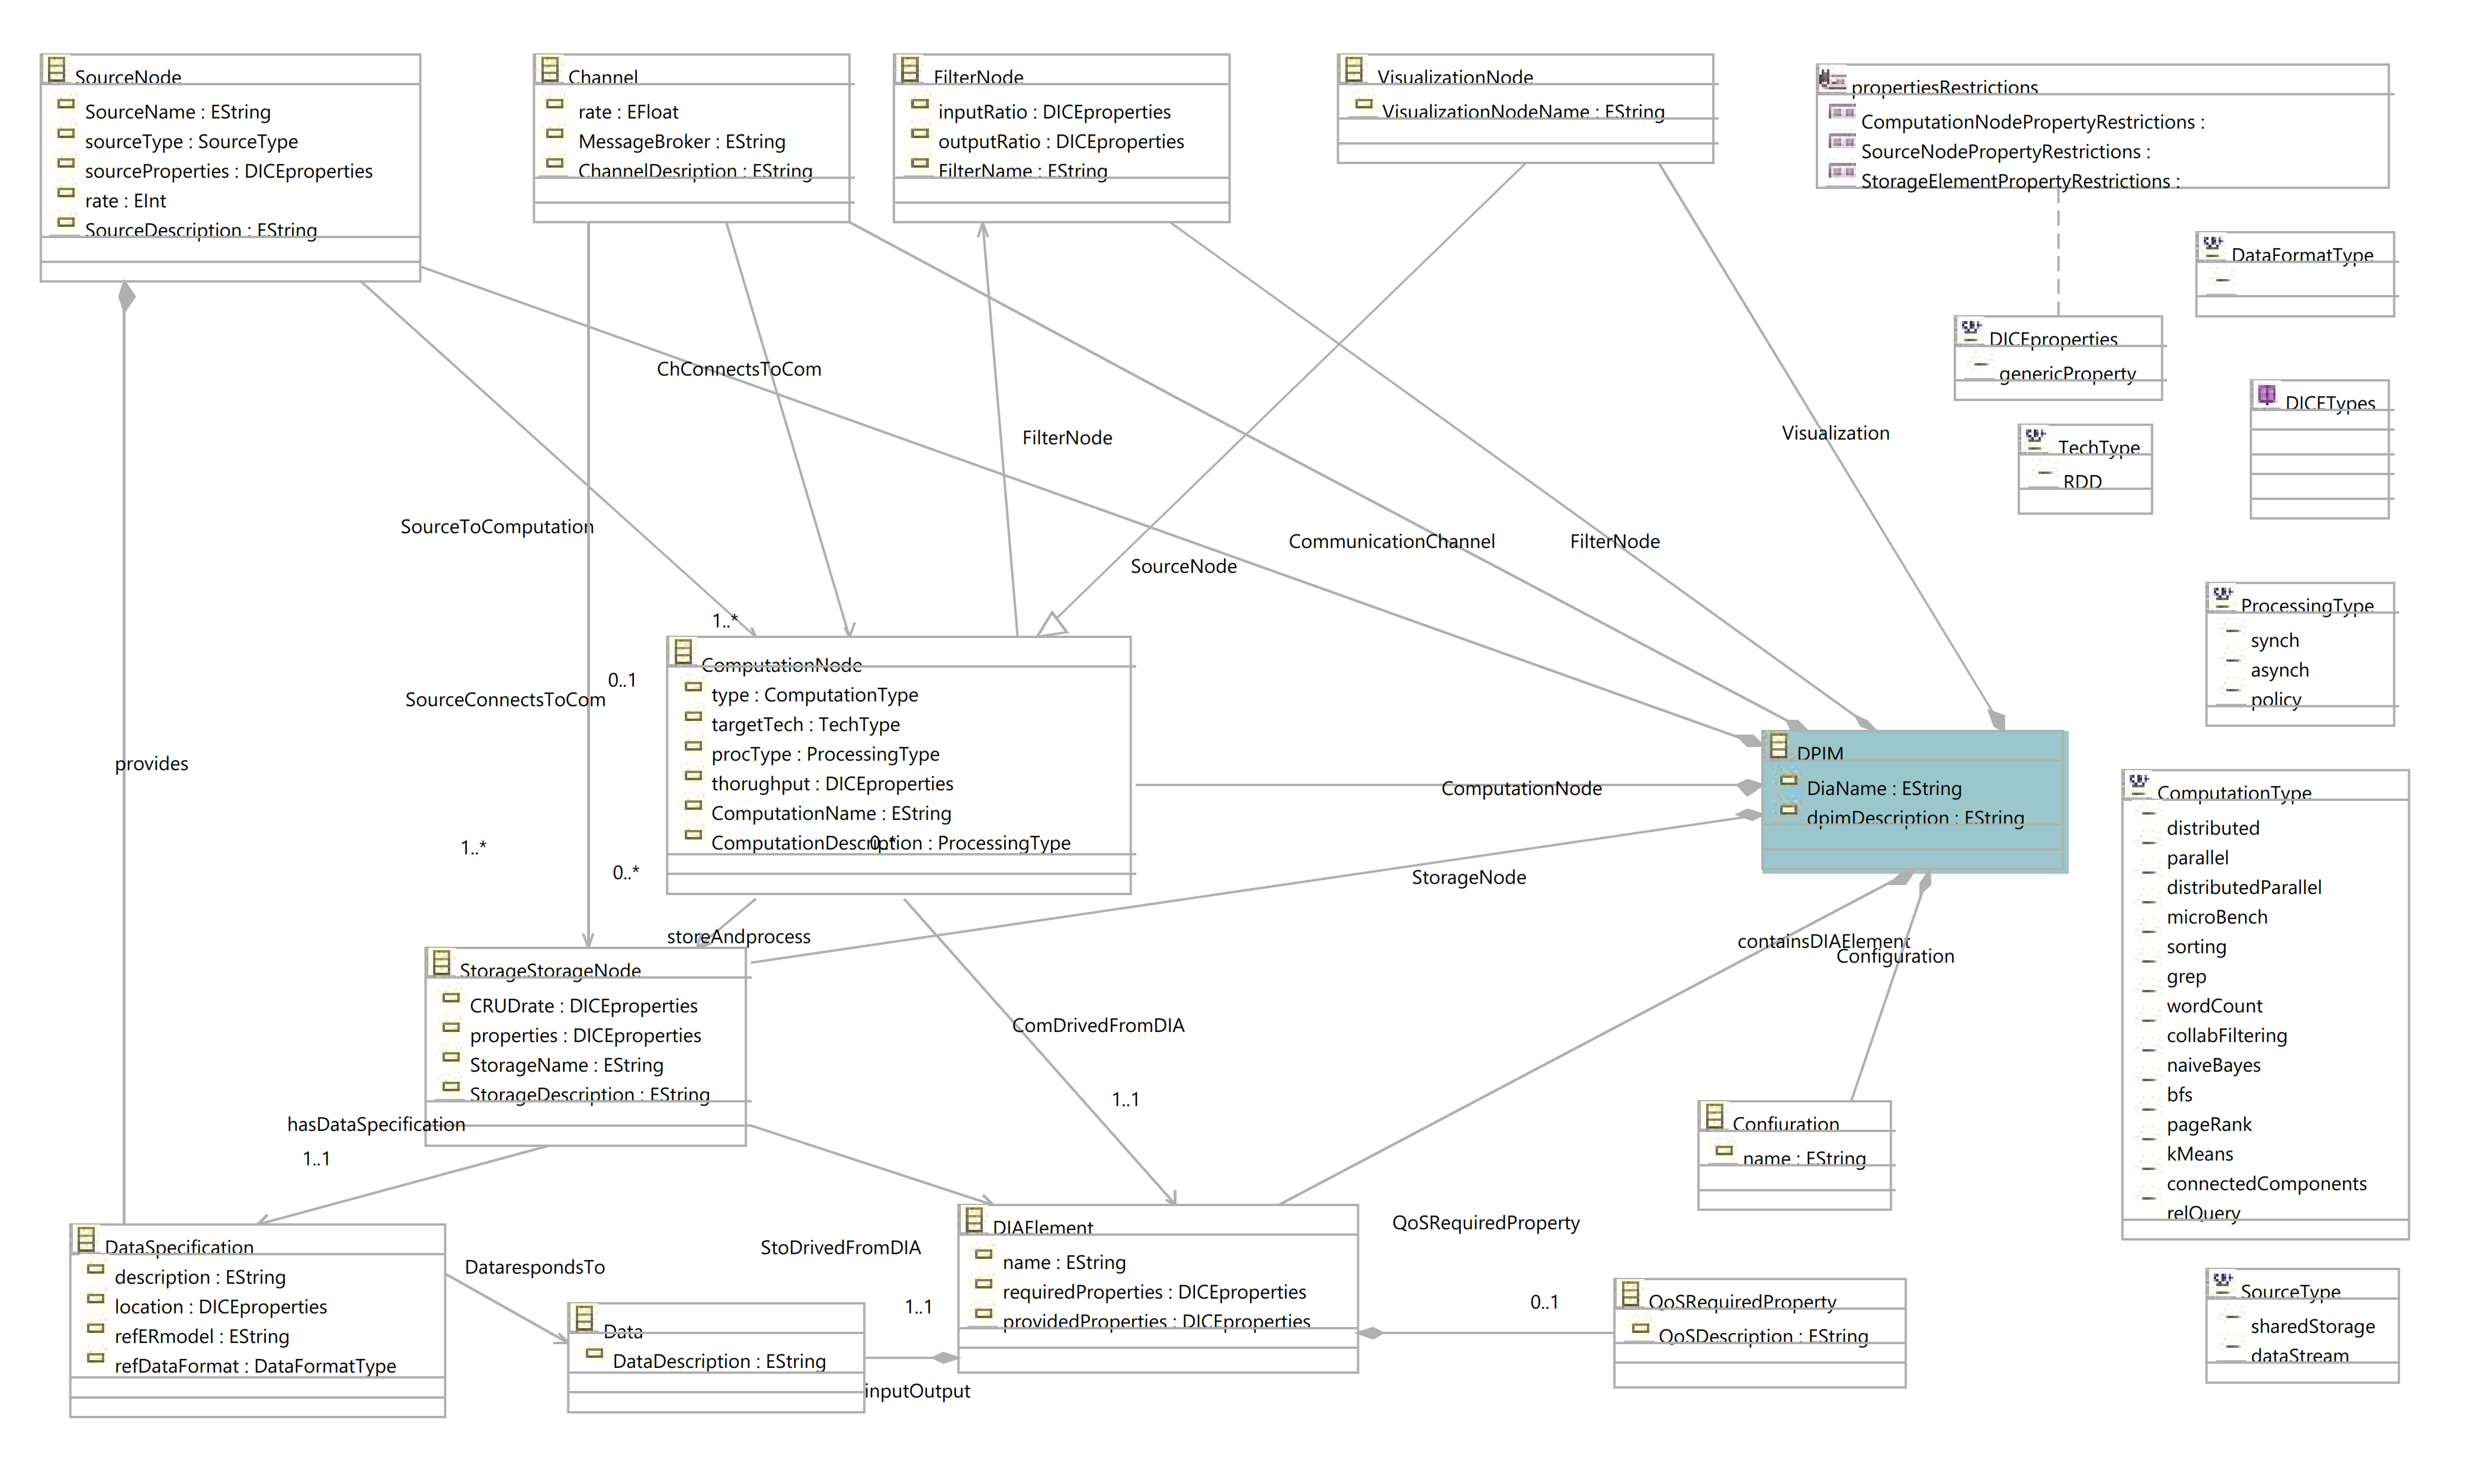
\includegraphics[width=\textwidth]{Images/11.png}
%\caption{\label{fig:metamodel2}DICE DPIM metamodel in portrait form.}
%\end{figure}

%Here is the command to refer to another element (section, figure, table, ...) in the document: \emph{As discussed in Section~\ref{sect:overview} and as shown in Figure~\ref{fig:metamodel}, ...}. Here is how to introduce a bibliographic citation~\cite{DAM}. Bibliographic references should be included in a \texttt{.bib} file. 
%
%Table generation is a bit complicated in Latex. You will soon become proficient, but to start you can rely on tools or external services. See for instance this \href{https://www.tablesgenerator.com}{https://www.tablesgenerator.com}. 


\subsection{Product Perspective}
Here we include scenarios and further details on the shared phenomena and a domain model (class diagrams and statecharts)


\begin{itemize}
\item
main objective of this system is to serve as an interface (intermediary?) between the farmers, agronomists, and policy makers. 
\item
intention is that this system will incorporate data-driven [blank] and include community focused [blank]? 
\item
this system will bridge the gap across these stakeholders with the goal for the telengana to to produce more effective and data-driven policies.
\item
since this is a big problem, with many involved people, people geographically spread out, etc this system provides an interface to that data can be shared and effectively used across users. 
\item
strengthen the cohesiveness of the policies generated and informed by data provided by users
\end{itemize}


\subsection{Product Functions}
Here we include the most important requirements
\par
Maybe add another table here?

% Let's format the requirements table here in a seperate file. We will very likely modify the requirements later on so saving it in a seperate file might make it easier to: 1) see where we need to make modifications and 2) identify formatting errors.
\begin{center}
\begin{longtable}{|c|>{\raggedright\arraybackslash}m{15cm}|}

    \hline
    \multicolumn{2}{|c|}{Begin}\\\hline
    \textbf{ID} & \textbf{Requirement}\\\hline
    \endfirsthead
    
    \hline
    \multicolumn{2}{|c|}{Cont.}\\\hline
    \textbf{ID} & \textbf{Requirement}\\\hline
    \endhead 
 
 
R1	& The system must allow the farmer to set the production types of their fields.\\\hline
R2	& The system must allow the farmer to set the position of their fields manually.\\\hline
R3	& The system must allow the farmer to set the position of their fields through their devices' GPS.\\\hline
R4	& The system must keep track of the data about farmers.\\\hline
R5	& The system must provide an interface to visualize data.\\\hline
R6	& The system must be able to analyze data and show statistics.\\\hline
R7	& The system must enable farmers to modify their production type.\\\hline
R8	& The system must enable farmers to report issues they may face. \\\hline
R9	& The system must allow the farmer to report production data at a frequency chosen by the farmer. \\\hline
R10	& The system must retrieve the weather forecast data from the data that the Telengana government collects.\\\hline
R11	& The system must show updated weather forecast data at most 5 minutes from which the data has been published by the Telengana government.\\\hline
R12	& The system must provide weather data that forecasts at least 3 days ahead.\\\hline
R13	& The system must allow agronomists to access weather forecast data specific to their responsible area.\\\hline
R14	& The system must allow farmers to access weather forecast data based on their GPS location or from the location of their farm on record.\\\hline
R15	& The system must provide an interface for farmers to request help and suggestions from other farmers.\\\hline
R16	& The system must provide an interface for farmers to receive help requests and receive suggestions sent to them from other farmers.\\\hline
R17	& The system must provide an interface for farmers to provide suggestions to other farmers.\\\hline
R18	& The system must provide an interface for farmers to respond to help requests sent to them from other farmers.\\\hline
R19	& The system must provide an interface for farmers to request help and suggestions from other agronomists.\\\hline
R20	& The system must provide an interface for agronomists to receive help requests sent to them from other farmers.\\\hline
R21	& The system must provide an interface for agronomists to respond to help requests sent to them from other farmers.\\\hline
R22	& The system must provide an interface for agronomists to provide suggestions to other farmers.\\\hline
R23	& The system must provide a forum interface.\\\hline
R24	& The system must allow the farmer to create discussion forums.\\\hline
R25	& The system must allow farmers to view all posts in the discussion forum.\\\hline
R26	& The system must allow farmers to post replies in the discussion forum.\\\hline
R27	& The system must keep track of all the forum discussion.\\\hline
R28	& The system must allow agronomists to specify their responsible geographic area.\\\hline
R29	& The system must allow agronomists to modify their responsible geographic area.\\\hline 
R30	& The system must allow agronomist to view the list of all farmers in their area. \\\hline
R31	& The system must provide an evaluation of farmers such that the evaluation reflects the quality and quantity of their crop production.\\\hline
R32	& The system must enable agronomists to access farmer evaluations from their specific area.\\\hline
R33	& The system updates farmers' evaluation when new data is available.\\\hline % (ie, new farmer event entries or after an agronomist visit, etc)
R34	& The system must provide an interface for daily plans.\\\hline
R35	& The system must recommend which farmers should be included in the agronomist's daily plan.\\\hline
R36	& The system must generate recommendations such that farmers are visited by their respective agronomists at least twice a year.\\\hline
R37	& The system must generate recommendations such that farmers with low evaluation are visited more often than twice a year.\\\hline
R38	& The system must allow agronomist to view the list of all farms to visit on a specific day.\\\hline
R39	& The system must allow agronomists to modify which farmers they visit in their plan.\\\hline
R40	& The system must allow agronomists to specify and modify the duration of the visits in their plan.\\\hline
R41	& The system must maintain a record of farmers who have been visited by their respective agronomists.\\\hline
R42	& The system must allow agronomists to modify the daily plan at the end of the day.\\\hline
R43	& The system must allow agronomists to confirm that the daily plan was executed that the end of that day.\\\hline
R44	& The system must not allow anymore modifications to the plan after the plan is confirmed by the agronomist.\\\hline
R45	& The system must only generate a new plan for a new day after the plan from the preceding day was confirmed by the agronomist.\\\hline
R46	& The system must allow Telengana’s policy makers to view the list of all farmers.\\\hline
R47	& The system must allow Telengana’s policy makers to view the performance and evaluation of the farmers.\\\hline
R48	& The system must allow Telengana’s policy makers to view the ranking of the farmers.\\\hline
R49	& The system must allow Telengana’s policy makers to view well-performing and poor-performing farmers.\\\hline
R50	& The system must allow Telengana’s policy makers to flag the farmers that need to be helped based on their performance.\\\hline
R51	& The system must designate each farmer a measure of support received by agronomists and other well-performing farmers.\\\hline
R52	& The system must allow policy makers to view the history of farmers’ performance/ evaluation.\\\hline
R53	& The system must allow Telengana policy makers to view this measure of support designated to each farmer.\\\hline
\end{longtable}
\end{center}


\subsection{User Characteristics}
\begin{flushleft}
This system expects three different types of users: farmer, agronomist, and policy maker.
\subsubsection{Farmer}
\subsubsection{Agronomist}
\subsubsection{Policy Maker}
A Telengana policy maker is a type of user that intends to use the DREAM system to drive policy decisions. Policy makers are mainly interested in accessing rankings and evaluations of all the farmers in the entire area as well as identifying broader trends in the data such as relating the community-provided support to production outcomes. Since policy makers have a more holistic view of the region, they use the DREAM system to configure metrics that are used to classify "well-performing" and "poor-performing" farmers based on rankings, evaluations, and data.\\
%\begin{itemize}
%\item
%mainly interested in seeing the evaluations generated by the system
%\item 
%may configure the metric to classify “well-performing” and “bad-performing” farmers based on rankings generated by system, evaluations from data, and natural/ climate circumstances specific to the year 
%\item
%will use the results seen on DREAM system to make policy decisions. These policy decisions exists outside of the system but will eventually affect the farmers and their production therefore may have an indirect after-effect on the data later inputted into the system
%\item
%the system should provide sufficient and clear data and analysis to enable telengana policy makers to make clear determinations of the efficacy of their policy decisions. 
%\end{itemize}
%



\end{flushleft}


\subsection{Assumptions, dependencies and constraints}
Here we include domain assumptions


% Assumptions Table
\newcounter{assum_counter}
\setcounter{assum_counter}{1}

\begin{table}
\centering
\caption{\label{tab:addOne{table_counter}}Domain Assumptions.}

\renewcommand{\arraystretch}{1.25}
\begin{tabular}{|l|>{\raggedright\arraybackslash}m{12cm}|} \hline
    \textbf{ID} & \textbf{Domain Assumption}\\\hline
	D\addOne{assum_counter} & Users must have a device connected to internet.\\\hline
	D\addOne{assum_counter} & To access to the system the user must have valid credentials.\\\hline
	D\addOne{assum_counter} & The data about weather forecast, the farmers and their production, the sensors, the agronomist are correct, complete and sent to the application. \\\hline
	D\addOne{assum_counter} & The user has granted permission for GPS, notifications and disk usage.\\\hline
	D\addOne{assum_counter} & Farmers have an existing system to quantify, track, and organize their production yields.\\\hline
	D\addOne{assum_counter} & Users can successfully operate an interactive application.\\\hline
	D\addOne{assum_counter} & Business competition will not influence the farmers' willingness to help.\\\hline
	D\addOne{assum_counter} & Farmers are willing to ask for help from other farmers and/or agronomists.\\\hline
	D\addOne{assum_counter} & Farmers have industry knowledge about fertilizers, crops, etc.\\\hline
	D\addOne{assum_counter} & Farmers are willing to interact with other farmers.\\\hline
	D\addOne{assum_counter} & Farmers can recognize issues and production abnormalities.\\\hline
	D\addOne{assum_counter} & Agronomists are assigned an area by their superiors.\\\hline
	D\addOne{assum_counter} & Agronomists can effectively manage an area assigned to them (ie, the agronomist is not overworked).\\\hline
	D\addOne{assum_counter} & Agronomists are experts in their field.\\\hline
	D\addOne{assum_counter} & Agronomists will be effective in addressing issues farmers face.\\\hline
	D\addOne{assum_counter} & Agronomists have access to an internet connection.\\\hline
	D\addOne{assum_counter} & Agronomists can successfully operate an interactive application.\\\hline
	D\addOne{assum_counter} & Weather forecast data is available.\\\hline
	D\addOne{assum_counter} & Weather forecast data is accurate.\\\hline
	D\addOne{assum_counter} & Farmers are not interested in meteorological changes that occur in less than 5 minutes.\\\hline
	D\addOne{assum_counter} & Agronomists are effective in determine performance based on various data points.\\\hline
	D\addOne{assum_counter} & Modifications to the daily plan are simple.\\\hline
	D\addOne{assum_counter} & confirmed plans actually happened /..... [better worded].\\\hline
	D\addOne{assum_counter} & Policy makers want to see the success of farmers in the form of production yields and crop quality.\\\hline
\end{tabular}
\end{table}


